\documentclass[12pt]{article}

\usepackage{answers}
\usepackage{setspace}
\usepackage{graphicx}
\usepackage{enumitem}
\usepackage{multicol}
\usepackage{mathrsfs}
\usepackage[margin=1in]{geometry} 
\usepackage{amsmath,amsthm,amssymb}
\usepackage{hyperref}

\hypersetup{
    colorlinks=true,
    linkcolor=blue,
    filecolor=magenta,      
    urlcolor=blue,
}

 
\newcommand{\N}{\mathbb{N}}
\newcommand{\Z}{\mathbb{Z}}
\newcommand{\C}{\mathbb{C}}
\newcommand{\R}{\mathbb{R}}

\DeclareMathOperator{\sech}{sech}
\DeclareMathOperator{\csch}{csch}
 
\newenvironment{theorem}[2][Theorem]{\begin{trivlist}
\item[\hskip \labelsep {\bfseries #1}\hskip \labelsep {\bfseries #2.}]}{\end{trivlist}}
\newenvironment{definition}[2][Definition]{\begin{trivlist}
\item[\hskip \labelsep {\bfseries #1}\hskip \labelsep {\bfseries #2.}]}{\end{trivlist}}
\newenvironment{proposition}[2][Proposition]{\begin{trivlist}
\item[\hskip \labelsep {\bfseries #1}\hskip \labelsep {\bfseries #2.}]}{\end{trivlist}}
\newenvironment{lemma}[2][Lemma]{\begin{trivlist}
\item[\hskip \labelsep {\bfseries #1}\hskip \labelsep {\bfseries #2.}]}{\end{trivlist}}
\newenvironment{exercise}[2][Exercise]{\begin{trivlist}
\item[\hskip \labelsep {\bfseries #1}\hskip \labelsep {\bfseries #2.}]}{\end{trivlist}}
\newenvironment{solution}[2][Solution]{\begin{trivlist}
\item[\hskip \labelsep {\bfseries #1}]}{\end{trivlist}}
\newenvironment{problem}[2][Problem]{\begin{trivlist}
\item[\hskip \labelsep {\bfseries #1}\hskip \labelsep {\bfseries #2.}]}{\end{trivlist}}
\newenvironment{question}[2][Question]{\begin{trivlist}
\item[\hskip \labelsep {\bfseries #1}\hskip \labelsep {\bfseries #2.}]}{\end{trivlist}}
\newenvironment{corollary}[2][Corollary]{\begin{trivlist}
\item[\hskip \labelsep {\bfseries #1}\hskip \labelsep {\bfseries #2.}]}{\end{trivlist}}
 
\begin{document}
 
% --------------------------------------------------------------
%                         Start here
% --------------------------------------------------------------
 
\title{Summary of Photodiode Sensitivity and Energy Consumption}
\author{Bryce Primavera}

\maketitle
\section{Motivation}
\quad The ultimate goal of this project will be to compare the performance and feasibility of various incoherent optoelectronic platforms for neuromorphic computing. Semiconductor photodetectors have already become a ubiquitous technology and are consequently a natural starting point for a whole class of potential optoelectronic neuromorphic hardware. This short summary seeks to accomplish two goals: (1) To determine the minimum optical power required for the detector to register an optical spiking event and (2) to analyze both the static and dynamic energy dissipation in a detector.

\section{Determining the Minimum Energy of a Spike}

\subsection{Photodetector Basics and Noise}
%\quad DERIVATION PRIMARILY DRAWN FROM THESE TWO SOURCES:
%\newline
%\hyperlink{http://ecee.colorado.edu/~bart/ecen6355/chapt-05.pdf}{http://ecee.colorado.edu/~bart/ecen6355/chapt-05.pdf} - section 5.1.2 pages 5.9-5.11
%\newline
%\hyperlink{https://users.physics.ox.ac.uk/~rtaylor/teaching/Opto_lecture5.pdf}{https://users.physics.ox.ac.uk/~rtaylor/teaching/Opto_lecture5.pdf} - section 4, pages 7-9
%\newline

\quad The most basic parameter for a photodetector is the \textit{responsivity}, $\mathcal{R}$. The responsivity is simply the ratio of photocurrent to input optical power. It is related to the external efficiency, $\eta$ as shown below:

\begin{equation}
    \mathcal{R} = \frac{q\eta\lambda}{hc}
\end{equation}

where $\lambda$ is the wavelength of the incoming light. $\eta$, and therefore $\mathcal{R}$, can be expected to be strong functions of wavelength. With responsivity defined, it is straightforward to predict the amount of photocurrent ($I_{ph}$) produced for a certain input optical power ($P_{opt}$):

\begin{equation}
    I_{ph} = \mathcal{R}P_{opt}
\end{equation}

In order to produce a measurable response, the photocurrent must be larger than the RMS fluctuations of the noise current. There are two primary sources of this noise in photodiodes - dark current noise and Johnson Noise from the load resistor. The noise from the dark current will be considered first. The RMS fluctuations can be given as:

\begin{equation}
    <I^{2}> = 2qI\Delta f
\end{equation}

$I$ is simply the total current flowing through the diode and $\Delta f$ is the bandwidth of the detector. This is already an interesting detail, as the noise can potentially be reduced by operating at a lower bandwidth (I guess this corresponds to something like integrating the signal?). For this paper, I will take the bandwidth to be 20 MHz, for sake of comparison with SOENS. In principle all sources of current - ideal diode current, SHR, band-to-band recombination, and photocurrent - should be included in $I$. 

We can approximate $I = I_{D} + I_{ph}$, where $I_{D}$ is the dark current. There is an additional Johnson Noise associated with the load resistor, $R_{L}$. This leads to a total noise, $I_{N}$ of:

\begin{equation}
    I_{N} = \sqrt{2qI\Delta f + \frac{4k_{B}T\Delta f}{R_{L}}}
\end{equation}

Equating the photocurrent with the RMS noise fluctuations gives an estimate of the bare minimum detectable optical power.

\begin{equation}
    P_{min} = \frac{I_N}{\mathcal{R}}
\end{equation}

Or in terms of the minimum necessary photocurrent, $I_{ph}$:

\begin{equation}
    I_{ph} = \sqrt{2q(I_D+I_{ph})\Delta f + \frac{4k_{B}T\Delta f}{R_{L}}
    }
\end{equation}

Solving the quadratic equation for $I_{ph}$ yields:

\begin{equation}
    I_{ph} = q\Delta f(1+\sqrt{1+\frac{2I_D+}{q\Delta f} +
    \frac{4k_BT}{q^2R_L\Delta f}})
\end{equation}

where $I_R = \sqrt{\frac{4k_{B}T\Delta f}{R_{L}}}$, the contribution to the noise current from the Johnson noise of the resistor. The minimum optical power, $P_{min}$ follows from the responsivity:

\begin{equation}
    P_{min} = \frac{I_{ph}}{\mathcal{R}}=
    \frac{q\Delta f}{\mathcal{R}}(1+\sqrt{1+\frac{2I_D}{q\Delta f} +
    \frac{4k_BT}{q^2R_L\Delta f}})
\end{equation}

The next task is to determine the appropriate temporal length of an optical spike. For a photodetector operating at its maximum rate, it suffices to use 1/$\Delta f$ as the duration of spike. Of course, this duration will likely be set by the speed of the LED, but for now I'm going to just assume that the bandwidth of our receiver circuit was designed to coincide with the bandwidth of the LED. In this case, with photon energy $E_{ph}$, the necessary number of photons per spike ($N$) is then:

\begin{equation}
    N = \frac{P_{min}}{E_{ph}\Delta f}
\end{equation}


A plot of the minimum number of photons per spike vs bandwidth is presented in Figure 1. From experimenting with some plausible parameters, it seems likely that noise will be dominated by the Johnson Noise in the load resistor. This noise can be reduced by utilizing a larger resistor. However, a larger $R_L$ will degrade the bandwidth of the circuit. A lower bandwidth requires the light source to be on for longer and increases the necessary optical power. In Figure 1, the color-coded vertical lines represent the maximum frequency that a 10pF photodiode could respond at. In fact, since the bandwidth is inversely proportional to $R_L$, it can be seen from equation 8 that in the resistor dominated noise regime, N will become independent of $R_L$. Fortunately, this bandwidth limit can be beaten by using a transimpedance amplifier as we will see in following sections.

\begin{figure}
    \centering
    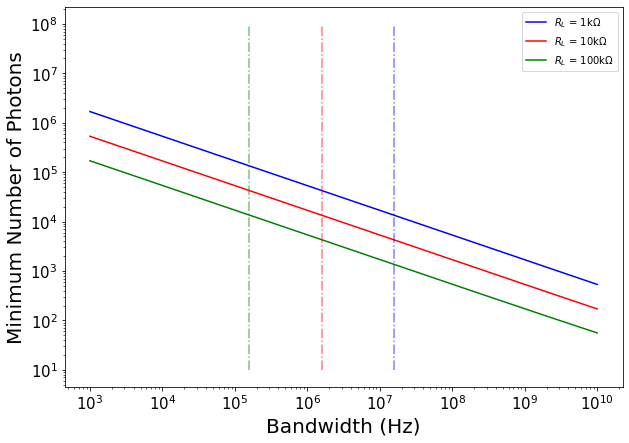
\includegraphics[width=15cm]{photon_V_BW.png}
    \caption{A plot of the minimum number of photons needed per spike as a function of Bandwidth. $I_D$ = 10nA, $\mathcal{R}$ = .5, and $\lambda$ = 1.3$\mu$m. The dotted vertical lines correspond to the maximum frequency achievable without a transimpedance amplifier for a 10pF photodiode. }
    \label{fig:my_label}
\end{figure}

Finally, we can also see a simple example of explicit temperature dependence. $I_D$ is a strong function of temperature and will play a role when we get to static power dissipation, but the Johnson noise in the resistors is more important for determining the minimum optical signal. It has a simple square root temperature dependence, which can be seen in figure 2.

\begin{figure}
    \centering
    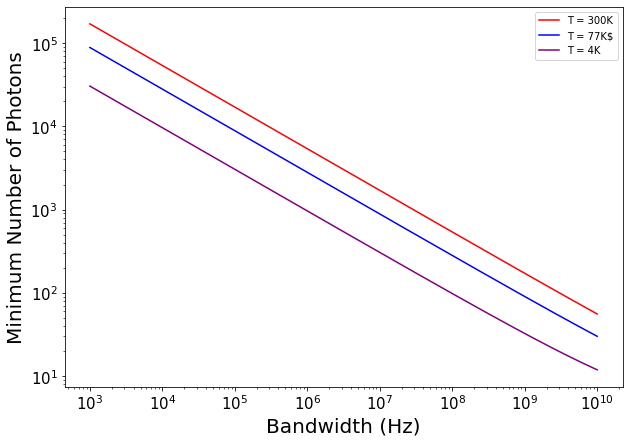
\includegraphics[width=15cm]{Temp_Photon_spike.png}
    \caption{Temperature dependence of the minimum optical signal. $R_L = 100k\Omega$}
    \label{fig:my_label}
\end{figure}

\subsection{Advantages (and Noise) of Transimpedance Amplifiers}

\end{document}
